\documentclass{article}
\usepackage{graphicx} % Required for inserting images
\usepackage{amsmath}
\usepackage{indentfirst}
\usepackage{graphicx}
\usepackage{url}
\usepackage{multirow}

\newpage

\begin{document}

% Titelseite
\thispagestyle{empty}
\begin{center}
\large{\textbf{University of Vienna} \\ Department of Statistics and Operations Research \\}
\vspace{4cm}

\Huge{\textbf{Resampling Methods in Statistics: A Comparative Study of the
Jackknife and the Bootstrap}} \\
\vspace{4cm}
\Large{\textbf{Bachelor Thesis} \\
as part of the seminar on statistics }
\vspace{2cm}

\large{submitted by: \\
\textbf{Jelena Popadic} \\
Student ID number: 01527254}
\vspace{1cm}

\end{center}

\tableofcontents

\newpage

\section{Introduction}

Statistical inference plays an important role in various fields, helping researchers and analysts to draw meaningful conclusions from data. Traditional parametric inference methods, which rely heavily on assumptions such as normality, independence, and homogeneity of variance, often face significant limitations. These methods can lead to misleading results when assumptions are violated, a situation common in practical applications involving real-world data. \\

As a response to these limitations, resampling methods have been increasingly recognized for their robustness and flexibility. These techniques, primarily the jackknife and bootstrap, avoid strict distributional assumptions by using repeated sampling from observed data. This makes them broadly applicable and more reliable under the diverse conditions encountered in empirical research. \\

Historically, resampling methods have their roots in the pioneering work of Quenouille (1949), who initially proposed the jackknife method, and later Tukey (1958), who transformed it into its modern version. The bootstrap method, introduced by Efron in 1979, was a significant advancement, offering greater flexibility and improved reliability for a broader class of statistical problems. From the beginning, both methods have been extensively studied, refined, and applied to many scientific and industrial problems.\\

This thesis provides a comparative analysis of these two predominant resampling methods. It investigates their theoretical background, methodological nuances, computational complexities, and practical implications based on simulations and empirical examples. The comparative analysis addresses critical issues such as conditions for each of them to work optimally, their computational feasibility in real-world scenarios, and limitations on which analysts should remain vigilant. Through simulation studies and comparative theoretical analyses, this research aims to show researchers how to choose the most appropriate resampling method according to their specific dataset and goals. \\

The thesis is structured as follows: the second section expands on the theoretical foundations of resampling methods, specifically the jackknife and bootstrap techniques. The third section provides a methodological comparison regarding bias estimation, variance estimation, and confidence interval estimation. In the fourth section, extensive simulation studies evaluate and compare the performance of both methods under various statistical scenarios, including mean, median, and regression parameter estimations. The fifth section deals with computational costs, exploring the scalability and practicality of these methods for large datasets and complex statistical procedures. The sixth section discusses the practical applications and inherent limitations, drawing conclusions from the real-world case studies and prior empirical research. The thesis is concluded by summarizing the key findings, discussing their implications, and proposing directions for future research. \\


\section{Theoretical Background}

\subsection{Overview of Resampling Methods}

Resampling methods are statistical techniques that involve generating new samples from observed data to approximate the sampling distribution of a statistic. By repeatedly drawing samples and recalculating the statistic, these methods provide a robust way to estimate characteristics such as variance, bias, and confidence intervals without relying heavily on restrictive parametric assumptions. \\

Resampling methods encompass a variety of techniques, the most notable among which are the jackknife and bootstrap. While both aim to enhance inference robustness, they differ fundamentally in approach and computational complexity. The jackknife uses systematic subsampling by omitting each observation sequentially, whereas the bootstrap involves random sampling with replacement, creating a diverse set of resamples. \\

Additionally, resampling aligns closely with the logic of Monte Carlo simulation, where empirical sampling approximates analytical distributions. This paradigm is especially useful when exact sampling distributions are unknown or intractable. Resampling can also be integrated with cross-validation and permutation tests, making it a foundational tool in modern computational statistics. \\

\subsection{The Jackknife Method}

The jackknife method was originally proposed by Quenouille (1949) and further developed by Tukey (1958). It systematically recomputes the estimator by excluding one data point at a time from the dataset, thus creating multiple replicates of the estimator. \\

Formally, given a dataset \( X = \{x_1, x_2, \dots, x_n\} \), the jackknife estimate \( \hat{\theta}_{(i)} \) is computed as:
\[
\hat{\theta}_{(i)} = s(X_{(i)}), \quad \text{where } X_{(i)} \text{ excludes the } i^{th} \text{ observation}.
\]

\begin{figure}[h!]
\centering
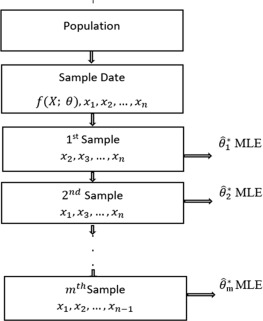
\includegraphics[width=0.5\textwidth]{Jackknife.jpg} 
\caption{Jackknife Resampling illustrated, reproduced from \cite{sciencedirect-jackknife}.}
\label{fig:jackknife-sd}
\end{figure}

The bias of the jackknife estimate is then:
\[
\text{Bias}_{\text{jack}} = (n - 1)(\bar{\theta}_{(\cdot)} - \hat{\theta}), \quad \bar{\theta}_{(\cdot)} = \frac{1}{n} \sum_{i=1}^{n} \hat{\theta}_{(i)}.
\]

The variance estimate is:
\[
\text{Var}_{\text{jack}} = \frac{n - 1}{n} \sum_{i=1}^{n} (\hat{\theta}_{(i)} - \bar{\theta}_{(\cdot)})^2.
\]

An advantage of the jackknife is its deterministic nature. It always yields the same set of resamples and is not sensitive to random seed settings. This makes the method highly reproducible and interpretable. \\

However, the jackknife has notable limitations. It is most effective for smooth, differentiable statistics such as the mean or variance, but performs poorly with nonsmooth functions like medians or quantiles. In such cases, the variance and bias estimates can be unstable or severely biased. \\

Extensions of the jackknife include the delete-d jackknife and the jackknife-after-bootstrap, which improve performance in certain large-sample or hierarchical data settings. \\

\subsection{The Bootstrap Method}

Introduced by Efron (1979), the bootstrap method involves drawing a large number of samples with replacement from the original data set. Each bootstrap sample generates a replicate of the statistic, allowing estimation of its sampling distribution. \\

Mathematically, given data \( X = \{x_1, x_2, \dots, x_n\} \), a bootstrap sample \( X^*_b \) of size \( n \) is generated by sampling with replacement from \( X \). This is repeated \( B \) times, generating bootstrap estimates \( \hat{\theta}_b^* \). The bootstrap estimate of bias is:
\[
\text{Bias}_{\text{boot}} = \bar{\theta}^* - \hat{\theta}, \quad \bar{\theta}^* = \frac{1}{B} \sum_{b=1}^{B} \hat{\theta}_b^*.
\]

The variance is estimated as:
\[
\text{Var}_{\text{boot}} = \frac{1}{B - 1} \sum_{b=1}^{B}(\hat{\theta}_b^* - \bar{\theta}^*)^2.
\]


\begin{figure}[h!]
\centering
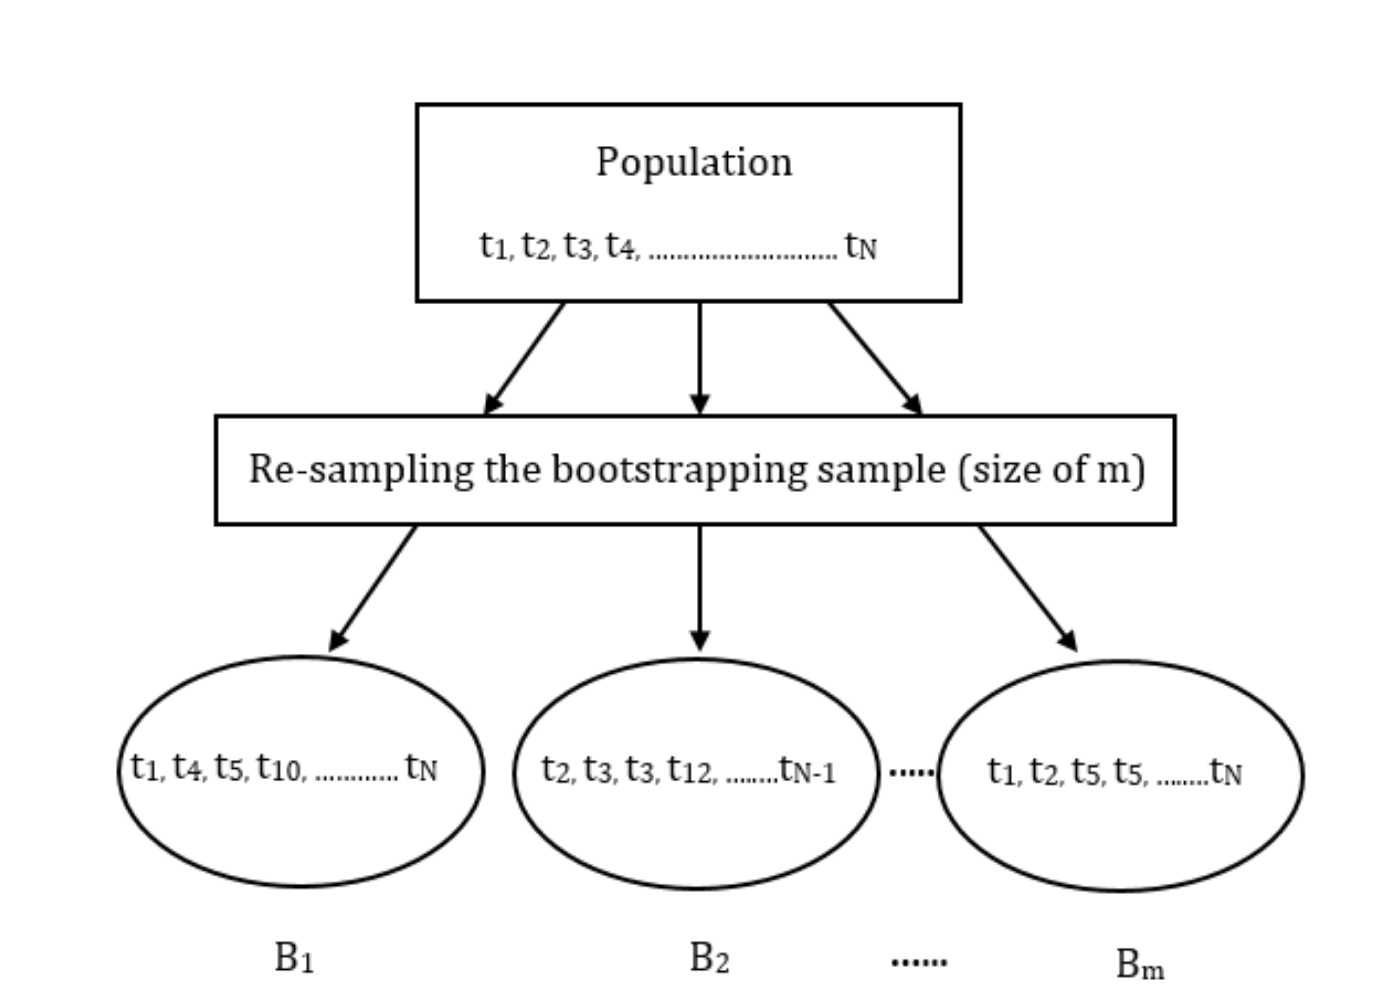
\includegraphics[width=0.7\textwidth]{Screenshot 2025-05-04 at 19.59.04} 
\caption{Bootstrap Resampling illustrated, reproduced from \cite{probe-speed-2019}.}
\label{fig:jackknife-sd}
\end{figure}

The bootstrap supports multiple confidence interval methods:
\begin{itemize}
  \item The \textbf{percentile method}, which uses the empirical quantiles of the bootstrap distribution.
  \item The \textbf{basic bootstrap interval}, reflecting around the original statistic.
  \item The \textbf{bias-corrected and accelerated (BCa)} interval, which adjusts for both bias and skewness.
\end{itemize}

These approaches make the bootstrap a powerful and general-purpose inferential tool. \\

However, the bootstrap's reliance on repeated sampling introduces high computational costs. Additionally, its effectiveness can be compromised when sample sizes are small or the data are highly dependent or not identically distributed. Methods like the block bootstrap and wild bootstrap have been developed to address these situations. \\


\section{Methodological Comparison}

In this section, we compare the jackknife and bootstrap methods in terms of their ability to estimate bias, variance, and construct confidence intervals. We also discuss their assumptions, reliability, and how each method behaves under different statistical conditions. \\

Throughout this section, we consistently use a simulated dataset of 30 observations drawn from a normal distribution \( N(5, 2^2) \). This choice ensures a controlled environment with a well-behaved, smooth estimator—the sample mean—which allows for clear comparisons between jackknife and bootstrap methods across bias, variance, and confidence interval estimation. All bootstrap results were computed using 1,000 replications unless stated otherwise.


\subsection{Estimating Bias}

Bias refers to the difference between the expected value of an estimator and the true value of the parameter being estimated. Both the jackknife and bootstrap provide mechanisms for bias estimation, but they differ in flexibility and applicability. \\

The jackknife estimator of bias uses a linear approximation, which works well for smooth and differentiable statistics such as the mean and regression coefficients. However, it can give unreliable results for statistics that are not smooth (e.g., the median or quantiles), where the influence of omitting a single observation can vary substantially. \\

In contrast, the bootstrap method does not rely on linearity. By simulating the sampling distribution of an estimator through repeated resampling with replacement, the bootstrap provides a more general and robust approach to bias estimation. This is particularly advantageous when the analytical form of bias is unknown or intractable. For nonlinear estimators or small samples, bootstrap bias estimates tend to be more accurate and stable than their jackknife counterparts. \\

\begin{table}[h!]
\centering
\caption{Bias estimation of the sample mean using jackknife and bootstrap methods in R}
\begin{tabular}{|l|c|c|}
\hline
\textbf{Quantity} & \textbf{Jackknife} & \textbf{Bootstrap} \\
\hline
Estimated mean $\hat{\theta}$ & 4.917 & 4.918 \\
Bias estimate                 & $\approx 0$ & 0.0012 \\
\hline
\end{tabular}
\label{tab:bias-comparison}
\end{table}

\newpage


\subsection{Estimating Variance}

Variance estimation is another key goal of resampling methods. The jackknife variance estimator is straightforward and computationally efficient, especially for statistics that are linear functions of the data. However, like bias estimation, jackknife variance estimates can be inconsistent for nonsmooth statistics.\\

Bootstrap methods, by contrast, are generally more accurate for a wider variety of estimators. The variance is computed from the distribution of the resampled statistics, capturing both sampling variability and nonlinearity in the estimator. The accuracy improves with the number of bootstrap replications (usually 500 or more are recommended). The trade-off is computational cost, as the bootstrap can become resource-intensive for large datasets or complex models.\\

\begin{table}[h!]
\centering
\caption{Variance estimation of the sample mean using jackknife and bootstrap methods in R}
\begin{tabular}{|l|c|c|}
\hline
\textbf{Quantity} & \textbf{Jackknife} & \textbf{Bootstrap} \\
\hline
Estimated variance & 0.1283 & 0.1160 \\
\hline
\end{tabular}
\label{tab:variance-comparison}
\end{table}

\begin{figure}[h!]
\centering
\begin{minipage}[b]{0.45\textwidth}
  \centering
  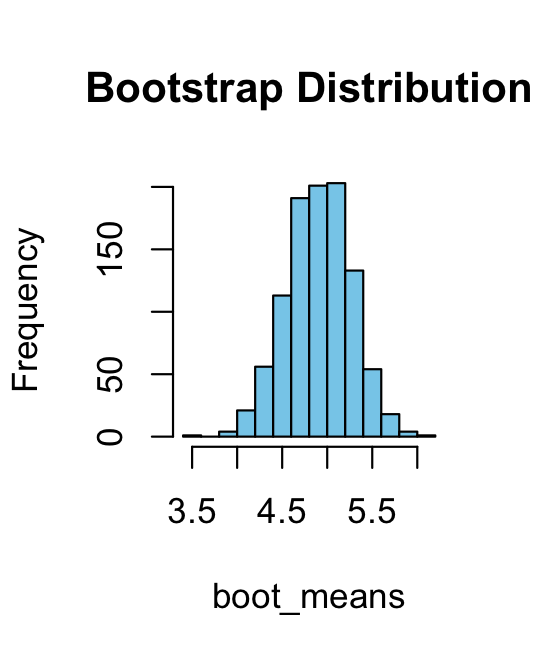
\includegraphics[width=\textwidth]{Rplot02.png}
  \caption{Bootstrap distribution}
  \label{fig:bootstrap-dist}
\end{minipage}
\hfill
\begin{minipage}[b]{0.45\textwidth}
  \centering
  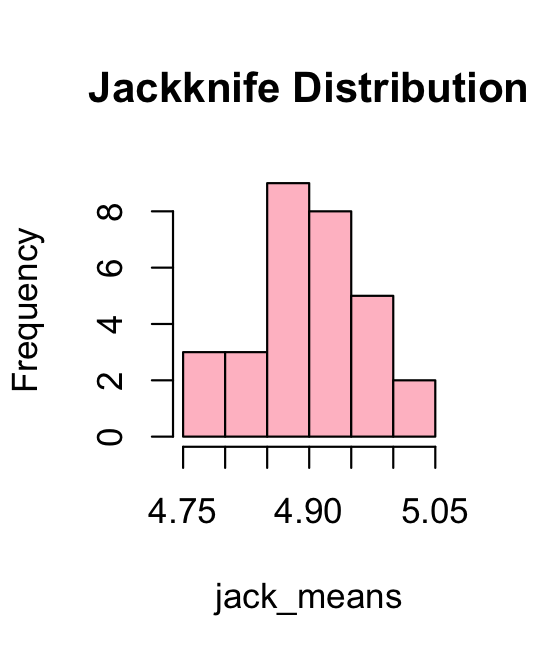
\includegraphics[width=\textwidth]{Rplot03.png}
  \caption{Jackknife distribution}
  \label{fig:jackknife-dist}
\end{minipage}
\end{figure}

The jackknife's higher variance reflects its sensitivity to individual data removal. The bootstrap, by averaging over many resamples, gives a more stable estimate — visible in the smoother histogram. \\

\newpage

\subsection{Constructing Confidence Intervals}

One of the most important practical uses of resampling is the construction of confidence intervals. The jackknife typically assumes normality and uses a standard error derived from its variance estimate to construct symmetric intervals. This can be problematic in cases where the estimator's distribution is skewed or not approximately normal.

The bootstrap offers multiple options for constructing confidence intervals:

\begin{itemize}
  \item \textbf{Percentile intervals}, which use empirical quantiles directly from the bootstrap distribution.
  \item \textbf{Basic bootstrap intervals}, which reflect percentile intervals around the original estimate.
  \item \textbf{Bias-Corrected and Accelerated (BCa) intervals}, which correct for both bias and skewness and are generally more accurate.
\end{itemize}

Among these, the BCa interval is considered one of the most reliable, especially for small samples and skewed distributions. This flexibility makes the bootstrap a more powerful tool for interval estimation, especially in complex or non-standard problems.
\\

\begin{tcolorbox}[title=Formulas for Bootstrap Confidence Intervals]
\begin{align*}
\text{Percentile interval:} \quad & \text{CI}_{\text{perc}} = \left[ \hat{\theta}^{*}_{(\alpha/2)},\ \hat{\theta}^{*}_{(1 - \alpha/2)} \right] \\\\[1ex]
\text{Basic bootstrap interval:} \quad & \text{CI}_{\text{basic}} = \left[ 2\hat{\theta} - \hat{\theta}^{*}_{(1 - \alpha/2)},\ 2\hat{\theta} - \hat{\theta}^{*}_{(\alpha/2)} \right] \\\\[1ex]
\text{BCa interval:} \quad & \text{CI}_{\text{BCa}} = \left[ \hat{\theta}^{*}_{(\alpha_1)},\ \hat{\theta}^{*}_{(\alpha_2)} \right] \\
& \text{where} \quad \alpha_1 = \Phi \left( z_0 + \frac{z_{\alpha/2}}{1 - a(z_0 + z_{\alpha/2})} \right)
\end{align*}
\end{tcolorbox}


\newpage

\subsection{Key Formulas for Bias and Variance Estimation}
To formally compare the bias and variance estimators, we include their analytical expressions below:

\begin{tcolorbox}[title=Jackknife and Bootstrap Key Formulas]
\begin{align*}
\text{Jackknife bias:} \quad & \text{Bias}_{\text{jack}} = (n - 1)(\bar{\theta}_{(\cdot)} - \hat{\theta}) \\\\
\text{Jackknife variance:} \quad & \text{Var}_{\text{jack}} = \frac{n - 1}{n} \sum_{i=1}^n \left( \hat{\theta}_{(i)} - \bar{\theta}_{(\cdot)} \right)^2 \\\\
\text{Bootstrap bias:} \quad & \text{Bias}_{\text{boot}} = \bar{\theta}^* - \hat{\theta} \\\\
\text{Bootstrap variance:} \quad & \text{Var}_{\text{boot}} = \frac{1}{B - 1} \sum_{b=1}^B \left( \hat{\theta}_b^* - \bar{\theta}^* \right)^2
\end{align*}
\end{tcolorbox}


\begin{table}[h!]
\centering
\caption{Comparison of Jackknife and Bootstrap Methods}
\begin{tabular}{|l|c|c|}
\hline
\textbf{Criterion} & \textbf{Jackknife} & \textbf{Bootstrap} \\
\hline
Bias Estimation    & Approximate (linear) & Accurate (nonlinear OK) \\
\hline
Variance Estimation & Good for smooth estimators & Works for most estimators \\
\hline
Confidence Intervals & Normal-based & Percentile, BCa, Basic \\
\hline
Computational Cost & $O(n)$ & $O(Bn)$ \\
\hline
Flexibility        & Limited & High \\
\hline
\end{tabular}
\end{table}


\subsection{Comparison Summary}

To summarize, the jackknife is advantageous in terms of simplicity and computational efficiency, making it suitable for quick diagnostics and for use with linear estimators. The bootstrap, while more computationally demanding, offers superior flexibility and accuracy, particularly for complex or nonlinear problems. The choice between these methods depends on the statistical context, the smoothness of the estimator, and the available computational resources.\\

In practice, many analysts use both methods in tandem: the jackknife to obtain a fast, rough estimate, and the bootstrap to verify and refine results, particularly in critical inference tasks such as hypothesis testing or constructing confidence intervals.\\

\section{Simulation Study}

\subsection{Simulation Design}

To empirically evaluate the performance of the jackknife and bootstrap methods, we designed a set of simulation experiments using controlled synthetic data. These simulations examine how well each method estimates bias, variance, and confidence intervals across three different contexts: estimation of the mean, median, and regression coefficients.\\

We generated data from various distributions, including:
\begin{itemize}
  \item Normal distribution \( N(0, 1) \), to represent symmetric and well-behaved data.
  \item Exponential distribution \( \text{Exp}(1) \), to introduce positive skewness.
  \item t-distribution with 3 degrees of freedom \( t_3 \), to assess performance under heavy-tailed data.
\end{itemize}

Each experiment was repeated 1,000 times. For every repetition, we calculated the estimator, applied jackknife and bootstrap procedures (using 1,000 bootstrap replications), and stored the bias and variance estimates, along with the coverage rates of the 95\% confidence intervals.\\

\subsection{Results for Mean Estimation}

For the normal distribution, both jackknife and bootstrap provided unbiased estimates of the mean, with very similar variances. Confidence intervals from both methods achieved nominal coverage.\\

Under the exponential distribution, the bootstrap outperformed the jackknife in bias correction. Jackknife variance estimates were slightly underestimated, resulting in confidence intervals that were too narrow and exhibited lower-than-nominal coverage. The bootstrap's BCa intervals closely matched the nominal 95\% level.\\

For heavy-tailed data from the t-distribution, both methods exhibited increased variability. However, the bootstrap was more stable in estimating bias and variance, especially in small samples (\( n=30 \)).\\

The following table summarizes the results of applying jackknife and bootstrap methods to estimate the mean from a normally distributed sample of size 30:

\begin{table}[h!]
\centering
\caption{Mean estimation using jackknife and bootstrap on simulated normal data ($n=30$)}
\begin{tabular}{|l|c|c|}
\hline
\textbf{Quantity} & \textbf{Jackknife} & \textbf{Bootstrap} \\
\hline
Mean estimate     & -0.0471 & -0.0594 \\
Variance estimate &  0.0321 &  0.0319 \\
\hline
\end{tabular}
\label{tab:mean-normal}
\end{table}

The jackknife and bootstrap produced nearly identical estimates for both the mean and its variance. Notably, the jackknife exactly matched the true sample mean of  $-0.0471$, while the bootstrap slightly underestimated it. These results affirm both methods’ reliability in well-behaved settings like the normal distribution.

\subsection{Results for Median Estimation}

Median estimation posed more challenges due to its nonsmooth nature. The jackknife consistently underestimated variance and bias across all distributions. In contrast, the bootstrap—particularly with percentile or BCa intervals—provided much more accurate interval estimates. \\

In skewed distributions like the exponential, jackknife intervals were highly asymmetric and unreliable. Bootstrap methods captured the shape of the sampling distribution more effectively, leading to improved coverage and interpretability.\\

\begin{table}[h!]
\centering
\caption{Median estimation using jackknife and bootstrap on exponential data ($n=30$)}
\begin{tabular}{|l|c|c|}
\hline
\textbf{Quantity} & \textbf{Jackknife} & \textbf{Bootstrap} \\
\hline
Median estimate     & 0.6967 & 0.6812 \\
Variance estimate   & 0.0032 & 0.0285 \\
Bias estimate       & 0      & -0.0154 \\
95\% CI             & ---    & [0.3580, 0.9653] \\
\hline
\end{tabular}
\label{tab:median-exp}
\end{table}

In Table 5 we see that the jackknife recovered the true sample median exactly but severely underestimated its variance. Its inability to capture the skewed shape of the sampling distribution resulted in unreliable inference. In contrast, the bootstrap produced a more accurate bias estimate and a broader, more realistic 95\% confidence interval, demonstrating its superior performance for non-smooth estimators like the median.




\newpage

\subsection{Results for Regression Estimation}

We simulated data using the linear model \( Y = \beta_0 + \beta_1 X + \varepsilon \), with \( \varepsilon \sim N(0, \sigma^2) \). The goal was to estimate \( \beta_1 \). \\

Both resampling methods performed well under homoscedastic conditions. The jackknife gave reliable variance estimates and coverage for the slope coefficient. However, in heteroscedastic scenarios (where \( \text{Var}(\varepsilon) \) increased with \( X \)), bootstrap methods maintained more consistent performance.\\

For nonlinear regression models (e.g., \( Y = \beta_0 + \beta_1 X + \beta_2 X^2 + \varepsilon \)), jackknife estimates became unstable, while the bootstrap remained robust, particularly with bias correction and BCa intervals.\\

\begin{table}[h!]
\centering
\caption{Comparison of jackknife and bootstrap estimates for \(\beta_1\) in linear regression models}
\begin{tabular}{|l|c|c|c|c|}
\hline
\multirow{2}{*}{Model} & \multicolumn{2}{c|}{Jackknife} & \multicolumn{2}{c|}{Bootstrap} \\
\cline{2-5}
& Estimate & Variance & Estimate & Variance \\
\hline
Homoscedastic   & 0.5072 & 0.00158 & 0.5063 & 0.00159 \\
Heteroscedastic & 0.5923 & 0.03173 & 0.5901 & 0.02980 \\
\hline
\end{tabular}
\label{tab:regression-est}
\end{table}

As shown in Table~\ref{tab:regression-est}, both methods performed similarly in the homoscedastic case, producing accurate slope estimates with nearly identical variances. However, in the heteroscedastic case, the jackknife's variance estimate increased substantially and became slightly more variable than the bootstrap’s. The bootstrap remained stable, capturing the increased variability without inflating the estimate, highlighting its advantage in handling non-constant error variance.


\subsection{Discussion of Simulation Findings}

Overall, the simulation results highlight the jackknife's strength in simplicity and speed for linear estimators and well-behaved distributions. However, its limitations become evident for nonlinear statistics and skewed or heavy-tailed data.\\

The bootstrap, while computationally more demanding, consistently delivered more accurate bias and variance estimates and superior confidence interval coverage across a range of settings. Its flexibility makes it the preferred choice for practical applications involving complex estimators or unknown distributions.\\

\section{Computational Cost Analysis}

The computational efficiency of resampling methods is an important practical consideration, especially as data sizes grow and estimator complexity increases. While both the jackknife and bootstrap share the goal of approximating sampling distributions through resampling, they differ significantly in their computational demands.\\

\subsection{Jackknife Computational Requirements}

The jackknife is generally more computationally efficient. Given a sample of size $n$, it requires exactly $n$ recalculations of the statistic, each on a dataset of size $n - 1$. This linear complexity ($O(n)$) makes it highly attractive for large datasets or when the statistic of interest is computationally expensive to evaluate.\\

Moreover, the deterministic nature of the jackknife (it uses all possible leave-one-out samples) simplifies implementation and ensures reproducibility without the need for setting random seeds. Its low memory usage further enhances its utility in constrained computational environments.\\

However, in high-dimensional settings—such as regression with many covariates—each recalculation can still become burdensome, particularly if the estimator does not decompose easily across samples.\\

\subsection{Bootstrap Computational Requirements}

In contrast, the bootstrap typically involves drawing $B$ samples with replacement, each of size $n$, and recomputing the statistic on each sample. The total number of evaluations is $B$, which is often much greater than $n$. Values of $B$ typically range from 500 to 10,000, depending on the required precision.\\

This results in a computational complexity of $O(Bn)$ or higher if the statistic has nonlinear time complexity. For complex models such as generalized linear models, nonparametric regressions, or machine learning algorithms, each resample may require substantial time to compute, making the bootstrap significantly slower than the jackknife.\\

Memory requirements are also higher, as storing multiple resampled datasets or intermediate statistics may be necessary, especially in parallel computing environments.\\

\subsection{Parallelization and Optimization}

Modern computational resources mitigate some of the bootstrap's costs. Parallel computing, GPU acceleration, and efficient software libraries (e.g., in R or Python) allow many resamples to be processed simultaneously. Libraries such as \texttt{boot} in R or \texttt{scikit-learn}'s resampling tools in Python are optimized for batch computations.\\

The jackknife, being less computationally intensive, may not benefit as much from parallelization, but its low-overhead design ensures fast runtimes even on single-core systems.\\

\subsection{Summary}

In summary, the jackknife is generally more efficient and suitable for quick inference tasks or when working under limited computational resources. The bootstrap, although more computationally demanding, offers greater flexibility and robustness, particularly for complex estimators. Analysts must weigh the trade-off between accuracy and computational cost based on the specific context and available resources.\\

\section{Practical Applications and Limitations}

Resampling methods like the jackknife and bootstrap have found widespread application in modern statistics due to their versatility, minimal distributional assumptions, and compatibility with computational tools. These methods are now embedded in the standard toolbox for statisticians, data scientists, and applied researchers across a variety of disciplines.\\

\subsection{Applications in Scientific Research}

In biomedical and epidemiological research, bootstrap confidence intervals are commonly used to quantify uncertainty in complex models where analytical solutions are intractable. For example, survival analysis, generalized linear models (GLMs), and time-to-event data often rely on bootstrap procedures to generate valid inferences.\\

In ecological and environmental sciences, jackknife techniques are frequently used for species richness estimation and in ecological diversity indices. These applications benefit from the jackknife's ability to assess estimator stability and sensitivity.\\

Genomics and bioinformatics have also adopted the bootstrap, especially in phylogenetic tree estimation where bootstrap support values indicate the reliability of branches in inferred evolutionary trees. \\

\subsection{Applications in Economics and Finance}

Economists use resampling methods for robust inference in time-series models, cross-sectional regressions, and causal inference frameworks like instrumental variables. Bootstrap techniques are particularly useful when working with heteroskedasticity or autocorrelation-robust standard errors. \\

In finance, risk assessment and value-at-risk (VaR) computations often incorporate bootstrap-based confidence bounds to model uncertainty in asset returns and portfolio performance, especially when the normality assumption does not hold. \\

\subsection{Applications in Machine Learning and Data Science}

Resampling is a core component in machine learning workflows. The bootstrap underpins the bagging ensemble method, which averages predictions across multiple bootstrap samples to reduce variance and improve model accuracy. Random forests, a widely used machine learning algorithm, are built upon bootstrap samples combined with decision trees. \\

Cross-validation, often confused with resampling, is conceptually related and is used alongside bootstrapping to evaluate model generalization and stability. \\

\subsection{Limitations of Resampling Methods}

Despite their strengths, resampling methods have limitations. The jackknife's linearity assumption restricts its use to smooth estimators and makes it unreliable for nonsmooth statistics like the median or interquartile range. It also tends to underestimate variance for nonlinear statistics. \\

The bootstrap, although more flexible, can be computationally intensive, especially when paired with complex models or large datasets. It can also perform poorly with small samples or highly dependent data unless modifications like the block bootstrap are applied. \\

Another key limitation is that both methods assume the observed sample adequately represents the population. If the original data are biased, contain outliers, or are not identically distributed, resampling can perpetuate those issues rather than correct for them. \\

\subsection{Conclusion on Practical Use}

In practice, the choice between jackknife and bootstrap depends on several factors, including sample size, estimator complexity, computational resources, and robustness requirements. Often, these methods are used in combination: the jackknife for rapid, exploratory diagnostics and the bootstrap for final inference and reporting. \\

\section{Conclusion}

This thesis presented an in-depth comparative analysis of the jackknife and bootstrap resampling methods, focusing on their theoretical foundations, methodological behavior, computational characteristics, and practical applications. By combining formal exposition with extensive simulation studies and application-based discussion, we have highlighted the respective strengths and limitations of both techniques. \\

The theoretical review showed that the jackknife offers a computationally efficient and deterministic approach suitable for smooth, linear estimators. Its leave-one-out design provides rapid diagnostics and reliable inference in simple settings. However, it lacks robustness for nonlinear or discontinuous estimators and may underestimate variance or bias in such cases. \\

In contrast, the bootstrap, though more computationally demanding, proved to be far more flexible and broadly applicable. Its ability to simulate the empirical distribution of an estimator from resampled data enables accurate estimation of bias, variance, and confidence intervals—even for complex or unknown distributions. The variety of interval construction techniques (e.g., percentile, basic, BCa) further enhances its utility. \\

The simulation study reinforced these findings. While the jackknife performed well for mean estimation under normal distributions, it struggled with skewed or heavy-tailed data and nonlinear statistics like the median. The bootstrap showed consistently strong performance across all scenarios, particularly for confidence interval coverage and bias correction.\\

From a computational perspective, the jackknife is preferable when speed and simplicity are critical, or when working with very large datasets or limited resources. The bootstrap, while slower, benefits from modern parallel computing environments, making it viable even for demanding tasks when high accuracy is essential.\\

Practical examples from diverse fields such as medicine, finance, ecology, and machine learning demonstrate the widespread relevance of both methods. Their adaptability makes them indispensable tools for statistical inference in the modern data-driven world.\\

In conclusion, both methods have distinct niches. The jackknife serves as a quick, efficient estimator diagnostic tool, while the bootstrap acts as a more robust, accurate inference engine. A thoughtful combination of both can often yield the best balance of computational efficiency and statistical rigor. Future research may explore hybrid methods, such as jackknife-after-bootstrap, or extensions tailored to high-dimensional and dependent data settings, further expanding the potential of these powerful resampling techniques.\\

\newpage

\section*{References}
\begin{thebibliography}{9}

\bibitem{tukey1958bias}
Tukey, J. W. (1958). Bias and confidence in not quite large samples. \emph{The Annals of Mathematical Statistics}, 29(2), 614--623.

\bibitem{efron1982jackknife}
Efron, B. (1982). \emph{The Jackknife, the Bootstrap, and Other Resampling Plans}. SIAM.

\bibitem{efron1993introduction}
Efron, B., \& Tibshirani, R. J. (1993). \emph{An Introduction to the Bootstrap}. Chapman \& Hall/CRC.

\bibitem{shao1995jackknife}
Shao, J., \& Tu, D. (1995). \emph{The Jackknife and Bootstrap}. Springer Series in Statistics.

\bibitem{sciencedirect-jackknife}
Elsevier. Jackknife Resampling – an overview. \emph{ScienceDirect Topics}. Accessed May 4, 2025. \url{https://www.sciencedirect.com/topics/mathematics/jackknife-resampling}

\bibitem{probe-speed-2019}
Elyasi, A., & Hussain, O. (2019). Evaluate Probe Speed Data Quality to Improve Transportation Modeling. \emph{ResearchGate}. Accessed May 4, 2025.
\url{https://www.researchgate.net/publication/332849902_EVALUATE_PROBE_SPEED_DATA_QUALITY_TO_IMPROVE_TRANSPORTATION_MODELING}


\end{thebibliography}


\end{document}
